\documentclass[conference]{IEEEtran}

% correct bad hyphenation here
\hyphenation{op-tical net-works semi-conduc-tor}

\usepackage{graphicx}
\graphicspath{{./img/}}


\begin{document}

\title{Report 1}

\author{
	\IEEEauthorblockN{Jun Huang}
	\IEEEauthorblockA{
		Gina Cody School of Engineering and Computer Science\\
		Concordia University\\
		Email: youyinnn@foxmail.com
	}
}
\maketitle

\begin{abstract}
	The abstract goes here.
\end{abstract}

\begin{IEEEkeywords}
	1-bit Adder, Hybird Adder, CMOS Technology,
\end{IEEEkeywords}

\section{Introduction}

...

An XOR-XNOR-based hybrid full adder design has been proposed\cite{20212210429416}
which uses an XOR-XNOR module combined with the carry-generation module and the sum-generation module.
As the designers discussed, it is a scalable and full-swing FA
with some performance improvements compared with several existing state-of-the-art FAs.

in section 2, xxx will be discussed...

% 列举其他找到的设计 但是并不在报告里讨论 因为设计的论文本身提供的信息在不做模拟的情况下难以放在同一个标准下进行比较 或者论文本身缺失了参数信息

\section{XOR-XNOR-based Hybrid Full Adder\cite{20212210429416}}

\subsection{Background}

The proposer of the design fist discussed how important ..

\subsection{Design}

This FA design contains three modules to perform a 1-bit full adder operation.
Firstly, an XOR-XNOR circuit will take original inputs \(A\) and \(B\) as its input and produce two signals,
one is from the XNOR gate marked as \(S_{xnor\_out}\) and the other is from the XOR gate marked as \( S_{xor\_out}\).
Then, a TG-based circuit as the second module will take both signal and the input carry \(C_{in}\) to calculate the \(Sum\)
while a third module will then use the \(C_{in}\) along with \(A\) and \(B\) and signals \(S_{xnor\_out}\) and \( S_{xor\_out}\) to generate the carry \(C_{out}\).

Fig. \ref{fig:fa1-bd} presents the block diagram of the design.

\begin{figure}[h!]
	\centering
	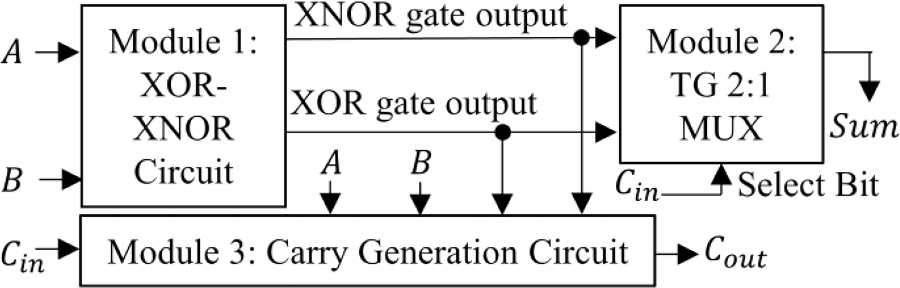
\includegraphics[width=2.7in]{fa1-block diagram.png}
	\caption{Block diagram of the XOR-XNOR-based FA}
	\label{fig:fa1-bd}
\end{figure}

\subsubsection{XOR-XNOR Circuit Design}



\section{Design B}

\section{Design C}

\section{Design D}

\section{Discussion}

\section{Conclusion}

\bibliographystyle{ieeetr}
\bibliography{bibliographies}
\end{document}
